%%%%%%%%%%%%%%%%%%%%%%%%%%%%%%%%%%%%%%%%%%%%%%%%%%%%%%%%%%%%%%%%%%%%%%%%%%%
%
% Template for a LaTex article in English.
%
%%%%%%%%%%%%%%%%%%%%%%%%%%%%%%%%%%%%%%%%%%%%%%%%%%%%%%%%%%%%%%%%%%%%%%%%%%%

\documentclass{article}

\usepackage[a4paper,margin=2cm]{geometry}

% AMS packages:
\usepackage{tikz}
\usetikzlibrary{arrows.meta}
\usepackage{environ}
\usepackage{amsmath, amsthm, amsfonts}
\usepackage{mathtools}
\usepackage[dvipsnames]{xcolor}
\usepackage[ruled,vlined,lined,boxed]{algorithm2e} 
\usepackage{xcolor}
\usepackage[framemethod=tikz]{mdframed}
\usepackage[english]{babel}
\usepackage[utf8]{inputenc}
\usepackage[T1]{fontenc}
\usepackage{stackrel}
\usepackage{hyperref}
\usepackage{enumitem}
\setlist[enumerate,1]{start=0}
\usepackage{comment}
% Solutions
%-----------------------------------------------------------------
\newif\ifshowsolutions
%\showsolutionstrue   % show solutions
\showsolutionsfalse % hide solutions
\ifshowsolutions
    \NewEnviron{solution}{%
        \par\medskip
        \color{blue}
        \noindent\textbf{Solution.}\quad
        \BODY
        \par\medskip
    }
\else
    \NewEnviron{solution}{}
\fi

% Commands
%-----------------------------------------------------------------
\newtheorem{thm}{Theorem}
\newtheorem{cor}[thm]{Corollary}
\newtheorem{lem}[thm]{Lemma}
\newtheorem{prop}[thm]{Proposition}
\theoremstyle{definition}
\newtheorem{defn}[thm]{Definition}
\newtheorem{assum}[thm]{Assumption}
\theoremstyle{remark}
\newtheorem{rem}[thm]{Remark}
\def\RR{\mathbb{R}}
\def\ZZ{\mathbb{Z}}
\def\NN{\mathbb{N}}
\newcommand{\abs}[1]{\left\vert#1\right\vert}
\renewcommand{\labelitemi}{$\vcenter{\hbox{\tiny$\bullet$}}$}
\DeclareMathOperator{\Jac}{Jac}

%-----------------------------------------------------------------

\usepackage[most]{tcolorbox}
\tcbuselibrary{breakable}
\newtcolorbox{boxA}{
    fontupper = \color{blue}, % font color
    boxrule = 0.8pt,
    colframe = blue,       % contour color (purple)
    colback = blue!10,   % interior color (light purple)
    rounded corners,
    arc = 5pt,               % corners roundness
    boxsep = 5pt,            % space between text and border
    left = 2pt,              % left padding
    right = 2pt,             % right padding
    top = 1pt,               % top padding
    bottom = 1pt             % bottom padding
}

\newtcolorbox{boxB}{
    fontupper = \color{ForestGreen}, % font color
    boxrule = 0.8pt,
    colframe = ForestGreen,       % contour color (purple)
    colback = green!10,   % interior color (light purple)
    rounded corners,
    arc = 5pt,               % corners roundness
    boxsep = 5pt,            % space between text and border
    left = 2pt,              % left padding
    right = 2pt,             % right padding
    top = 1pt,               % top padding
    bottom = 1pt             % bottom padding
}

\newtcolorbox{boxC}{
    breakable,
    fontupper = \color{black}, % font color
    boxrule = 0.8pt,
    colframe = gray,       % contour color (purple)
    colback = white,   % interior color (light purple)
    rounded corners,
    arc = 5pt,               % corners roundness
    boxsep = 5pt,            % space between text and border
    left = 2pt,              % left padding
    right = 2pt,             % right padding
    top = 1pt,               % top padding
    bottom = 1pt             % bottom padding
}

\colorlet{colorSolution}{blue}

\begin{document}
\noindent\textbf{Course:} LINMA2472: Algorithms in Data Science
\\[0.2cm]
\noindent\textbf{Professor:} Benoît Legat (benoit.legat@uclouvain.be)
\\[0.2cm]
\noindent\textbf{Teaching assistants:} Adeline Colson (adeline.colson@uclouvain.be), Sophie Lequeu (sophie.lequeu@uclouvain.be), Bastien Massion (bastien.massion@uclouvain.be)
\\[0.2cm]

\Large \noindent\textbf{Reverse Automatic Differentiation and the Adjoint Jacobian} \\

\normalsize \noindent\textbf{List of exercises}

\begin{boxA}
    Reminder: Let function $F$ be defined by the composition
    \[
    F \coloneqq f_L \circ f_{L-1} \circ \cdots \circ f_1.
    \]
    Then by the Chain Rule,
    \[
    J_F(x)
    =
    J_{f_L}(s_{L-1})\cdots J_{f_2}(s_1) \cdot J_{f_1}(s_0),
    \]
    where $s_0 \coloneqq x$ and $s_k \coloneqq f_k(s_{k-1})$.
\end{boxA}

\begin{boxB}
    Application to Automatic Differentiation: 
    \begin{itemize}
        \item Forward AD: 
        \[
        J_F(x) \cdot u
        =
        J_{f_L}(s_{L-1})\cdots J_{f_2}(s_1) \cdot J_{f_1}(s_0) \cdot u. \qquad \text{(JVP)}
        \]
        We compute
        \begin{equation*}
            t_k \coloneqq J_{f_k}(s_{k-1}) \cdot t_{k-1}, \qquad \text{for } k = 1, \dots, L \text{ and  with } t_0 \coloneqq u.
        \end{equation*}
        \item Reverse AD: 
        \[
        J_F(x)^\top \cdot v
        =
          J_{f_1}(s_0)^\top \cdot J_{f_2}(s_1)^\top \cdots J_{f_L}(s_{L-1})^\top \cdot v. \qquad \text{(VJP)}
        \]
        We compute
        \begin{equation*}
            r_k \coloneqq J_{f_{k+1}}(s_{k})^\top \cdot r_{k+1}, \qquad \text{for } k = L-1, \dots, 0 \text{ and  with } r_L \coloneqq v.
            \end{equation*}
    \end{itemize}
    In AD, for computational and storage reasons, we consider Jacobians (and Adjoint Jacobians) as \textbf{Linear Maps}, and not as matrices.
\end{boxB}
    
\begin{boxA}
    Reminder: The adjoint of a linear map $\mathcal{A}$ for a given scalar product
    $\langle \cdot, \cdot \rangle$ is the linear map $\mathcal{A}^*$ such that
    \[
        \forall x,y, \qquad
        \langle \mathcal{A}(x), y \rangle
        =
        \langle x, \mathcal{A}^*(y) \rangle.
    \]
\end{boxA}\vspace{0.3cm}

1. \textbf{Adjoint Jacobian of matrix multiplication on the right}. \vspace{0.2cm}\\
Consider the elementary operation 
\[F_1: \mathbb{R}^{m \times n} \rightarrow \mathbb{R}^{m \times p}, \quad F_1(X) = XB,\]
for some $B\in \mathbb{R}^{n \times p}$ and the Frobenius inner product $\langle X, Y\rangle = \operatorname{tr}(XY^\top)$. \vspace{0.2cm}\\
The action of the Jacobian of this elementary operation on a perturbation
$V$ is given by $J_{F_1}(X)[V] = VB$,
which can be viewed as the linear map
$\mathcal{A}(V)=VB$ applied on the direction $V$. Using the definition above, find the Adjoint  Jacobian of operation $F_1$. \vspace{0.2cm}\\
\[
\setlength{\fboxsep}{8pt}
\fbox{$\displaystyle \mathcal{A}^*(Y) = \hspace{3cm}$}
\] \\
\begin{solution}
Using the definition of adjoint recalled above and the cyclic property of the trace, we find
\[
    \forall X, Y, \qquad \langle \mathcal{A}(X), Y \rangle = \langle XB, Y \rangle = \operatorname{tr}(XBY^\top) = \operatorname{tr}(X(YB^\top)^\top) = \langle X, YB^\top \rangle = \langle X, \mathcal{A}^*(Y) \rangle, 
\]
where therefore
\[
    \mathcal{A}^*(Y)=YB^\top.
\]
\end{solution}

2. \textbf{Adjoint Jacobian of the Hadamard product}. \vspace{0.2cm}\\
Consider the elementary operation
\[
F_2: \mathbb{R}^{m \times n} \rightarrow \mathbb{R}^{m \times n},
\qquad
F_2(X) = X \odot B,
\]
for some $B\in \mathbb{R}^{m \times n}$, where $\odot$ denotes the Hadamard
(element-wise) product, and the Frobenius inner product is given by $\langle X, Y\rangle = \operatorname{tr}(XY^\top)$.
\vspace{0.2cm}\\
The Jacobian in the direction $V$ can be viewed as a linear map, $J_{F_2}(X)[V] = \mathcal{A}(V)$. Find the expression of this linear map. 
Then, using the definition above, find the adjoint Jacobian of the operation $F_2$.
\vspace{0.2cm}\\
\[
\setlength{\fboxsep}{8pt}
\fbox{$\displaystyle \mathcal{A}^*(Y) = \hspace{3cm}$}
\] \\
\begin{solution}
First, the Jacobian in the direction $V$ is
\[
    J_{F_2}(X)[V]
    =
    \left.\frac{\mathrm{d}}{\mathrm{d}t}
    F_2(X+tV)\right|_{t=0}
    =
    \left.\frac{\mathrm{d}}{\mathrm{d}t}
    \bigl((X+tV)\odot B\bigr)\right|_{t=0}
    =
    V\odot B.
\]
Hence, the corresponding linear map is
\[
    \mathcal{A}(V)=V\odot B.
\]
Using the definition and the properties of the Frobenius inner product, we find
\[
    \forall X, Y, \qquad
    \langle \mathcal{A}(X), Y \rangle
    =
    \langle X \odot B, Y \rangle
    =
    \sum_{i,j} X_{ij} B_{ij} Y_{ij}
    =
    \sum_{i,j} X_{ij} (Y \odot B)_{ij}
    =
    \langle X, Y \odot B \rangle
    =
    \langle X, \mathcal{A}^*(Y) \rangle,
\]
where therefore
\[
    \mathcal{A}^*(Y)=Y\odot B = \mathcal{A}(Y).
\]
\end{solution}

3. \textbf{Adjoint Jacobian of the broadcasted square}. \vspace{0.2cm}\\
Consider the elementary operation
\[
F_3: \mathbb{R}^{m \times n} \rightarrow \mathbb{R}^{m \times n},
\qquad
F_3(X) = X^{\odot 2},
\]
where $X^{\odot 2}$ denotes the element-wise square of $X$, and the Frobenius
inner product is given by $\langle X, Y\rangle = \operatorname{tr}(XY^\top)$.
\vspace{0.2cm}\\
The Jacobian in the direction $V$ can be viewed as a linear map,
$J_{F_3}(X)[V] = \mathcal{A}_X(V)$. Find the expression of this linear map.
Then, using the definition above, find the adjoint Jacobian of the operation $F_3$.
\vspace{0.2cm}\\
\[
\setlength{\fboxsep}{8pt}
\fbox{$\displaystyle \mathcal{A}_X^*(Y) = \hspace{3cm}$}
\]
\begin{solution}
First, the Jacobian in the direction $V$ is
\[
    J_F(X)[V]
    =
    \left.\frac{\mathrm{d}}{\mathrm{d}t}
    F(X+tV)\right|_{t=0}
    =
    \left.\frac{\mathrm{d}}{\mathrm{d}t}
    (X+tV)^{\odot 2}\right|_{t=0}
    =
    2X\odot V.
\]
Hence, the corresponding linear map is
\[
    \mathcal{A}_X(V)=2X\odot V.
\]
Using the definition of adjoint recalled above and the properties of the
Frobenius inner product, we find
\[
    \forall H, Y, \qquad
    \langle \mathcal{A}_X(H), Y \rangle
    =
    \langle 2X \odot H, Y \rangle
    =
    \sum_{i,j} 2X_{ij}H_{ij}Y_{ij}
    =
    \sum_{i,j} H_{ij}(2X_{ij}Y_{ij})
    =
    \langle H, 2X \odot Y \rangle
    =
    \langle H, \mathcal{A}_X^*(Y) \rangle,
\]
where therefore
\[
    \mathcal{A}_X^*(Y)=2X\odot Y = \mathcal{A}_X(Y).
\]
\end{solution}

4. \textbf{Adjoint Jacobian of the sum of all matrix elements}. \vspace{0.2cm}\\
Consider the elementary operation
\[
F_4: \mathbb{R}^{m \times n} \rightarrow \mathbb{R},
\qquad
F_4(X) = \sum_{i=1}^{m}\sum_{j=1}^{n} X_{ij},
\]
where $\mathbb{R}^{m \times n}$ is equipped with the Frobenius inner product
$\langle X, Y\rangle = \operatorname{tr}(XY^\top)$ and $\mathbb{R}$ with the
usual scalar product.
\vspace{0.2cm}\\
The Jacobian in the direction $V$ can be viewed as a linear map,
$J_{F_4}(X)[V] = \mathcal{A}(V)$. Find the expression of this linear map.
Then, using the definition above, find the adjoint Jacobian of the operation $F_4$.
\vspace{0.2cm}\\
\[
\setlength{\fboxsep}{8pt}
\fbox{$\displaystyle \mathcal{A}^*(y) = \hspace{3cm}$}
\]
\begin{solution}
First, the Jacobian in the direction $V$ is
\[
    J_{F_4}(X)[V]
    =
    \left.\frac{\mathrm{d}}{\mathrm{d}t}
    F_4(X+tV)\right|_{t=0}
    =
    \left.\frac{\mathrm{d}}{\mathrm{d}t}
    \left(
    \sum_{i=1}^{m}\sum_{j=1}^{n}(X_{ij}+tV_{ij})
    \right)\right|_{t=0}
    =
    \sum_{i=1}^{m}\sum_{j=1}^{n}V_{ij}.
\]
Hence, the corresponding linear map is
\[
    \mathcal{A}(V)
    =
    \sum_{i=1}^{m}\sum_{j=1}^{n}V_{ij}.
\]
Using the definition of adjoint recalled above, we find
\[
    \forall V, y, \qquad
    \langle \mathcal{A}(V), y \rangle
    =
    y \sum_{i=1}^{m}\sum_{j=1}^{n} V_{ij}
    =
    \sum_{i=1}^{m}\sum_{j=1}^{n} V_{ij} y
    =
    \left\langle V, y\mathbf{1}_{m\times n} \right\rangle
    =
    \langle V, \mathcal{A}^*(y) \rangle,
\]
where $\mathbf{1}_{m\times n}$ denotes the matrix whose entries are all equal to $1$.
Therefore,
\[
    \mathcal{A}^*(y)
    =
    y\mathbf{1}_{m\times n}.
\]
\end{solution}

5. \textbf{Adjoint Jacobian of the softmax}. \vspace{0.2cm}\\
Consider the elementary operation
    \[
    F_4: \mathbb{R}^{1 \times n} \rightarrow \mathbb{R}^{1 \times n},
    \qquad
    F_4(X) = \operatorname{softmax}(X),
    \]
    where
    \[
    \bigl(F_4(X)\bigr)_i
    =
    \frac{e^{X_i}}{\sum_{j=1}^n e^{X_j}},
    \]
    and $\mathbb{R}^{1 \times n}$ is equipped with the Frobenius inner product
    $\langle X,Y\rangle=\operatorname{tr}(XY^\top)$.
    \vspace{0.2cm}\\
    Let
    \[
    S=\operatorname{softmax}(X).
    \]
    The Jacobian in the direction $V$ can be viewed as a linear map,
    $J_{F_4}(X)[V]=\mathcal{A}_X(V)$.
    Find the expression of this linear map.
    Then, using the definition above, find the adjoint Jacobian of the operation
    $F_4$.
    \vspace{0.2cm}\\
    
    \[
    \setlength{\fboxsep}{8pt}
    \fbox{$\displaystyle \mathcal{A}_X^*(Y) = \hspace{3cm}$}
    \]
    
    \begin{solution}
        Let
        \[
            S=\operatorname{softmax}(X).
        \]
        For each component, the Jacobian in the direction $V$ is
        \[
        \begin{aligned}
            \bigl(J_{F_4}(X)[V]\bigr)_i
            &=
            \left.
            \frac{\mathrm{d}}{\mathrm{d}t}
            \frac{e^{X_i+tV_i}}
            {\sum_{j=1}^n e^{X_j+tV_j}}
            \right|_{t=0} \\
            &= \frac{
            e^{X_i}V_i\sum_{j=1}^n e^{X_j}
            -
            e^{X_i}\sum_{j=1}^n e^{X_j}V_j
            }{
            \left(\sum_{j=1}^n e^{X_j}\right)^2
            } \\[1mm]
            &=
            S_iV_i
            -
            S_i\sum_{j=1}^n S_jV_j.
        \end{aligned}
        \]
        Therefore,
        \[
            J_{F_4}(X)[V]
            =
            S\odot V-\langle S,V\rangle S.
        \]
        Hence, the corresponding linear map is
        \[
            \mathcal{A}_X(V)
            =
            S\odot V-\langle S,V\rangle S.
        \]
        Using the definition of adjoint recalled above, we find
        \[
        \begin{aligned}
            \langle \mathcal{A}_X(V),Y\rangle
            &=
            \left\langle
            S\odot V-\langle S,V\rangle S,Y
            \right\rangle \\
            &=
            \langle S\odot V,Y\rangle
            -
            \langle S,V\rangle\langle S,Y\rangle \\
            &=
            \langle V,S\odot Y\rangle
            -
            \left\langle
            V,\langle S,Y\rangle S
            \right\rangle \\
            &=
            \left\langle
            V,
            S\odot Y-\langle S,Y\rangle S
            \right\rangle \\
            &=
            \langle V,\mathcal{A}_X^*(Y)\rangle.
        \end{aligned}
        \]
        Therefore,
        \[
            \mathcal{A}_X^*(Y)
            =
            S\odot Y-\langle S,Y\rangle S
            =
            \mathcal{A}_X(Y).
        \]
        It can also be written as 
        \[
            \mathcal{A}_X^*(Y)
            =
            S\odot (Y-\langle S,Y\rangle \mathbf{1}^\top).
        \]
    \end{solution}
    \vspace{0.3cm}

6. \textbf{FlashAttention in Transformers}. \vspace{0.2cm}\\
In this exercise, we introduce the attention mechanism used in transformers, then derive a memory-efficient variant known as \emph{FlashAttention}. You will complete a Julia implementation in which some lines have been removed. \\
Let $Q,K,V \in \mathbb{R}^{n \times d}$ be the query, key, and value matrices. The standard scaled dot-product attention is defined by
\[
S = \frac{QK^\top}{\sqrt{d}}, \qquad
P = \operatorname{softmax}(S) \ \text{(row-wise)}, \qquad
O = PV.
\]
The naive implementation materializes the two $n \times n$ matrices $S$ and $P$, which becomes expensive when $n$ is large. FlashAttention avoids storing these matrices. Instead, it computes the output in tiles, stores only the output $O$ and one scalar per row
\[
L_i = \log\!\sum_j \exp(S_{ij}),
\]
and recomputes the needed blocks during the backward pass.

\begin{itemize}
    \item \textbf{Attention.}
    Explain why the naive implementation of attention requires $O(n^2)$ memory.
    Then write the formula for the backward pass with respect to $Q$, $K$, and $V$, based on the expression graph given hereafter.
    
    \begin{center}
        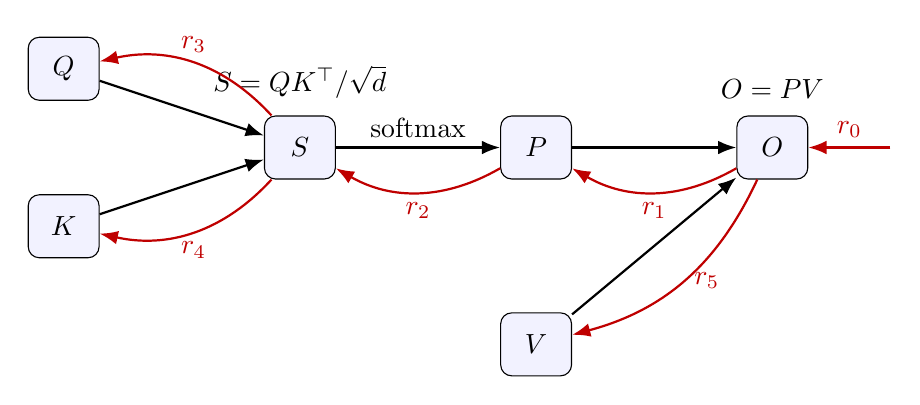
\begin{tikzpicture}[
        >=Latex,
        varnode/.style={
            draw, rounded corners,
            minimum width=9mm, minimum height=8mm,
            fill=blue!5
        },
        forward/.style={->, thick},
        backward/.style={->, thick, red!75!black},
        every edge quotes/.style={font=\small}
    ]   
        \node[varnode] (Q) at (0, 1) {$Q$};
        \node[varnode] (K) at (0,-1) {$K$};
        \node[varnode] (S) at (3, 0) {$S$};
        \node[varnode] (P) at (6, 0) {$P$};
        \node[varnode] (O) at (9, 0) {$O$};
        \node[varnode] (V) at (6,-2.5) {$V$};
    
        \draw[forward] (Q) -- (S);
        \draw[forward] (K) -- (S);
        \draw[forward] (S) --
            node[above] {$\operatorname{softmax}$} (P);
        \draw[forward] (P) -- (O);
        \draw[forward] (V) -- (O);
    
        \node[above=5mm] at (S) {$S=QK^\top/\sqrt d$};
        \node[above=5mm] at (O) {$O=PV$};
    
        \draw[backward] (10.5,0) --
            node[above] {$r_0$} (O);
    
        \draw[backward] (O) to[bend left=30]
            node[below] {$r_1$} (P);
        \draw[backward] (P) to[bend left=30]
            node[below] {$r_2$} (S);
        \draw[backward] (S) to[bend right=30]
            node[above] {$r_3$} (Q);
        \draw[backward] (S) to[bend left=30]
            node[below] {$r_4$} (K);
        \draw[backward] (O) to[bend left=25]
            node[right] {$r_5$} (V);
        \end{tikzpicture}
    \end{center}
        
    \begin{solution}
        The naive attention computation forms
        \[
        S=\frac{QK^\top}{\sqrt d},\qquad
        P=\operatorname{softmax}(S)\quad\text{(row-wise)},\qquad
        O=PV.
        \]
        Since both $S$ and $P$ are dense $n\times n$ matrices, the memory cost is $O(n^2)$.
    
        For the backward pass, if $r_0$ is the reverse tangent (at node $O$), then
        \[
        r_5=P^\top r_0,\qquad
        r_1=r_0\,V^\top,\qquad
        r_2=P\odot\bigl(r_1-((P\odot r_1)\mathbf{1})\mathbf{1}^\top\bigr).
        \]
        Note each line of $D := (P\odot r_1)\mathbf{1}$ is $D_i := \left[(P\odot r_1)\mathbf{1}\right]_i = \sum_j P_{ij} (r_1)_{ij}$ (see exercise $5$ for the adjoint jacobian of the softmax function applied to a row vector). Finally
        \[
        r_3=\frac{r_2\,K}{\sqrt d},\qquad
        r_4=\frac{r_2^\top Q}{\sqrt d}.
        \]
    \end{solution}

    \item \textbf{The key identity.}
    In the backward pass, when computing $r_2$, the naive softmax derivative contains the term
    \[
    D_i = \sum_j P_{ij}\,(r_1)_{ij}.
    \]
    Show that this term can also be written as
    \[
    D_i = \sum_k (r_0)_{ik} O_{ik}.
    \]
    Explain why this identity makes it possible to compute the backward pass without storing $P$.

    \begin{solution}
        Start from
        \[
        D_i=\sum_j P_{ij}(r_1)_{ij}.
        \]
        Since $r_1=r_0\,V^\top$, we have
        \[
        (r_1)_{ij}=\sum_k (r_0)_{ik}V_{jk}.
        \]
        Therefore
        \[
        D_i=\sum_j P_{ij}\sum_k (r_0)_{ik}V_{jk}
        =\sum_k (r_0)_{ik}\sum_j P_{ij}V_{jk}.
        \]
        But
        \[
        O_{ik}=\sum_j P_{ij}V_{jk},
        \]
        so
        \[
        D_i=\sum_k (r_0)_{ik}O_{ik}.
        \]
        Hence
        \[
        D=\operatorname{rowsum}(r_0\odot O),
        \]
        which only requires $O$ and $r_0$, not $P$.
    \end{solution}
\end{itemize}

\begin{boxC}
    \textbf{\textcolor{gray}{Note about the implementation, for the following two questions.}} \\
    
    To compute attention without storing the full matrices $S$ and $P$,
    we process the keys and values tile by tile, accumulating the numerator
    and denominator of
    \[
    O_{i,:}
    =
    \frac{\sum_j \exp(S_{ij})V_{j,:}}
            {\sum_j \exp(S_{ij})}.
    \]
    
    \textbf{For numerical stability}, we subtract a row-wise maximum $m_i$
    from the scores before exponentiating. This leaves the ratio
    unchanged, since the factor $\exp(-m_i)$ cancels between the
    numerator and denominator. Because the scores are computed tile by tile, we maintain a
    \emph{running maximum}. After processing a set of key indices $J$,
    the running variables satisfy
    \[
    m_i = \max_{j\in J} S_{ij},
    \qquad
    l_i = \sum_{j\in J} \exp(S_{ij}-m_i),
    \qquad
    \widetilde{O}_{i,:}
    = \sum_{j\in J} \exp(S_{ij}-m_i)V_{j,:}.
    \]
    The unnormalized accumulator $\widetilde{O}$ is stored in the
    variable \texttt{O} in the code.
    
    When a new tile increases the maximum from $m_i$ to
    $m_i^{\mathrm{new}}$, we rescale the previous contributions using
    \[
    \exp(S_{ij}-m_i^{\mathrm{new}})
    =
    \exp(m_i-m_i^{\mathrm{new}})\exp(S_{ij}-m_i).
    \]
    Thus, we multiply both running sums by
    $\exp(m_i-m_i^{\mathrm{new}})$ before adding the contributions
    of the new tile, computed relative to the new maximum.
    
    After processing all tiles, we recover
    \[
    O_{i,:} = \frac{\widetilde{O}_{i,:}}{l_i},
    \qquad
    L_i = m_i+\log(l_i).
    \]
    Tiling avoids storing the full attention matrices, while the
    running maximum keeps the exponential computations numerically stable.
\end{boxC}

\begin{itemize}
    \item \textbf{FlashAttention forward pass.}
        In the file \texttt{flash.jl}, the function \texttt{attn\_flash\_fwd} computes the forward pass by iterating over tiles of keys and values.
        Complete the missing parts of the algorithm so that the function returns the correct output $O$ and the vector $L$.

        \begin{solution}
            The forward pass processes the keys and values by tiles. For each block `j`,
            it computes
            \[
            S_{\mathrm{block}}=\frac{QK_{j}^\top}{\sqrt d},
            \]
            updates the running row-wise maximum `m`, rescales the running sum `l`, and
            accumulates the output `O`. At the end,
            \[
            O\leftarrow O./l,\qquad L=m+\log(l).
            \]
        
            So the missing logic is:
            \begin{itemize}
                \item initialize `O = 0`, `m = -Inf`, `l = 0`;
                \item for each tile:
                \begin{itemize}
                    \item compute `S = Q * K[jj, :]' ./ sqrt(d)`;
                    \item compute `mnew = max.(m, vec(maximum(S, dims=2)))`;
                    \item compute `Pblk = exp.(S .- mnew)`;
                    \item compute `corr = exp.(m .- mnew)`;
                    \item update `l` and `O`;
                    \item set `m .= mnew`;
                \end{itemize}
                \item normalize with `O ./= l` and return `O, L`.
            \end{itemize}
        \end{solution}
    
    \item \textbf{FlashAttention backward pass.}
        In the file \texttt{flash.jl}, the function \texttt{attn\_flash\_back} recomputes each tile during the backward pass.
        Fill in the missing lines so that the function returns the gradients
        \[
        r_3,\quad r_4,\quad r_5.
        \]
        Your implementation should use the previously stored values $O$ and $L$, and it should never materialize the full attention matrix.

        \begin{solution}
            First compute
            \[
            D=\operatorname{rowsum}(r_0\odot O).
            \]
            Then for each tile `j`,
            \[
            S_{\mathrm{block}}=\frac{QK_{j}^\top}{\sqrt d},\qquad
            P_{\mathrm{block}}=\exp(S_{\mathrm{block}}-L),
            \]
            and update
            \[
            (r_5)_{j} \mathrel{+}= P_{\mathrm{block}}^\top r_0,
            \]
            \[
            r_{1, \mathrm{block}} = r_0\,V_{j}^\top,
            \]
            \[
            r_{2, \mathrm{block}} = P_{\mathrm{block}}\odot(r_{1, \mathrm{block}}-D),
            \]
            \[
            r_3 \mathrel{+}= \frac{r_{2, \mathrm{block}}K_{j}}{\sqrt d},\qquad
            (r_4)_{j} \mathrel{+}= \frac{r_{2, \mathrm{block}}^\top Q}{\sqrt d}.
            \]
        
            This returns the same gradients as the naive backward pass, without storing the
            full attention matrix.
        \end{solution}
    
        \item \textbf{Discussion.}
        Use the provided benchmark to compare naive attention and FlashAttention as a function of sequence length.
        Explain why the flash version can be slower for small $n$, even though it uses less memory.
        \begin{solution}
            FlashAttention can be slower for small $n$ because it does extra work:
            it recomputes blocks of scores in the backward pass, manages tiled updates and
            rescaling, and trades arithmetic for reduced memory traffic.
        
            At small sequence lengths, that overhead can dominate, while the naive version
            benefits from simpler dense matrix operations. The flash version becomes
            advantageous when $n$ is large enough that the $O(n^2)$ memory traffic of the
            naive implementation becomes the bottleneck.
        \end{solution}
    \end{itemize}

7. \textbf{Adapted from Exam of August 2026}. \vspace{0.2cm}\\
Let
\[
    f(x,Q)=x^\top Qx-x^\top b,
    \qquad
    x=\begin{bmatrix}1\\2\end{bmatrix},
    \qquad
    Q=\begin{bmatrix}1&2\\3&4\end{bmatrix},
    \qquad
    b = \begin{bmatrix}3\\0
    \end{bmatrix}
\]
where $Q$ is not assumed to be symmetric. We evaluate this function as
\[
    s=Qx, \qquad t=x^\top s, \qquad g = x^\top b, \qquad f=t-g.
\]

\begin{itemize}
    \item Draw the corresponding expression graph and indicate the forward values. An arrow points from each argument to the operation that uses it.
    \item Starting with $\bar f=\partial f/\partial f=1$, perform the backward
    pass. Give the order in which you process the operation nodes and show how
    the adjoint of $x$ accumulates its three contributions.
    \begin{solution}
        A valid reverse topological order is $f$, $g$, $t$, then $s$. From
        $f=t-g$, we obtain
        \[
            \bar t \mathrel{+}=\bar f=1.
        \]
        and
        \[
            \bar g \mathrel{+}= (-1) \cdot \bar f=-1.
        \]
        From $g=x^\top b$, we obtain
        \[
            \bar x \mathrel{+}=\bar g\,b
                =\begin{bmatrix}-3\\0\end{bmatrix},
            \qquad
            \bar b \mathrel{+}=\bar g\,x
                =\begin{bmatrix}-1\\-2\end{bmatrix}.
        \]
        From $t=x^\top s$, we obtain
        \[
            \bar x \mathrel{+}=\bar t\,s
                =\begin{bmatrix}5\\11\end{bmatrix},
            \qquad
            \bar s \mathrel{+}=\bar t\,x
                =\begin{bmatrix}1\\2\end{bmatrix}.
        \]
        Finally, from $s=Qx$,
        \[
            \bar Q \mathrel{+}=\bar s x^\top
                =\begin{bmatrix}1&2\\2&4\end{bmatrix},
            \qquad
            \bar x \mathrel{+}=Q^\top\bar s
                =\begin{bmatrix}7\\10\end{bmatrix}.
        \]
        Hence the three contributions to $\bar x$ accumulate to
        \[
            \bar x=
            \begin{bmatrix}-3\\0\end{bmatrix}
            +\begin{bmatrix}5\\11\end{bmatrix}
            +\begin{bmatrix}7\\10\end{bmatrix}
            =\begin{bmatrix}9\\21\end{bmatrix}.
        \]
    \end{solution}
    
    \item Give $\nabla_x f$, $\nabla_Q f$ and $\nabla_b f$, first as formulas valid for
    arbitrary $x$, $Q$ and $b$, and then at the values above. Why does
    $\nabla_Q f$ have rank one whenever $x\ne0$?\begin{solution}
        The input adjoints give
        \[
            \nabla_x f=(Q+Q^\top)x - b,
            \qquad
            \nabla_Q f=xx^\top
            \qquad
            \nabla_b f=-x.
        \]
        At the specified values,
        \[
            \nabla_x f=\begin{bmatrix}12\\21\end{bmatrix},
            \qquad
            \nabla_Q f=\begin{bmatrix}1&2\\2&4\end{bmatrix}, 
            \qquad
            \nabla_b f=\begin{bmatrix}-3\\0\end{bmatrix}.
        \]
        For every vector $v$, $(xx^\top)v=x(x^\top v)$ belongs to
        $\operatorname{span}(x)$. Thus $xx^\top$ has rank at most one, and
        its rank is exactly one when $x\ne0$.
    \end{solution}

    \item More generally, suppose that a scalar-valued function has many
    inputs. To compute its full gradient, which mode is usually preferable:
    forward or reverse? Briefly justify your answer.
    \begin{solution}
        Reverse mode is usually preferable. A single reverse pass computes
        the derivative of the scalar output with respect to every input,
        whereas forward mode generally requires one pass per input direction.
    \end{solution}
\end{itemize}

\end{document}
